% ----------------------------------------------------------
% FIGURE: HR@tau response surface
% ----------------------------------------------------------
\begin{figure}[htbp]
\centering
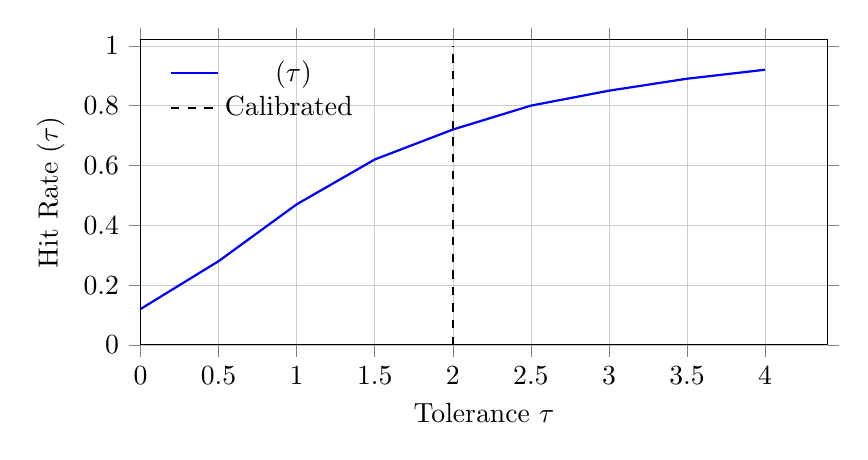
\begin{tikzpicture}
\begin{axis}[
    width=0.85\textwidth,
    height=0.45\textwidth,
    xlabel={Tolerance $\tau$},
    ylabel={Hit Rate $\HR(\tau)$},
    ymin=0, ymax=1.02,
    xmin=0,
    grid=both,
    major grid style={line width=.2pt, draw=gray!40},
    minor grid style={line width=.1pt, draw=gray!20},
    tick align=outside,
    legend style={
        at={(0.03,0.97)},
        anchor=north west,
        draw=none,
        fill=none
    }
]

% --- HR@tau curve (illustrative shape) ---
\addplot[
    thick,
    blue
] coordinates {
    (0.0, 0.12)
    (0.5, 0.28)
    (1.0, 0.47)
    (1.5, 0.62)
    (2.0, 0.72)
    (2.5, 0.80)
    (3.0, 0.85)
    (3.5, 0.89)
    (4.0, 0.92)
};

\addlegendentry{$\HR(\tau)$}

% --- Calibrated tau (example) ---
\addplot[
    dashed,
    thick,
    black
] coordinates {
    (2.0, 0.0)
    (2.0, 1.0)
};

\addlegendentry{Calibrated $\taustar$}

\end{axis}
\end{tikzpicture}

\caption{
Illustrative HR@$\tau$ response surface as a function of tolerance.
The curve shows the monotone increase in hit rate as the acceptable error band
widens, with diminishing marginal gains beyond moderate tolerance levels.
The calibrated tolerance $\taustar$ is selected within a stable region of the
response surface, balancing coverage improvement against tolerance inflation.
}
\label{fig:hrtau_response_surface}
\end{figure}